\section{Hệ quản trị Cơ sở dữ liệu (Database)}
Cơ sở dữ liệu là thành phần nền tảng có vai trò lưu trữ, quản lý và truy xuất thông tin
phục vụ các nghiệp vụ cốt lõi của ứng dụng. Việc triển khai hợp lý giúp đảm bảo tính
toàn vẹn, nhất quán và an toàn dữ liệu.
\subsection{PostgreSQL}
PostgreSQL (thường gọi là Postgres) là một Hệ quản trị cơ sở dữ liệu quan hệ đối tượng (Object-Relational Database Management System - ORDBMS) mã nguồn mở mạnh mẽ, Express.js đã trở thành framework backend phổ biến
nhất trong hệ sinh thái Node.js nhờ kiến trúc đơn giản, hiệu suất cao và khả
năng mở rộng dễ dàng. Nó nổi tiếng về độ tin cậy, tính năng mạnh mẽ và hiệu suất cao.
\begin{itemize}
    \item \textbf{Tuân thủ ACID:} Đảm bảo tính toàn vẹn dữ liệu ở mức cao nhất (Atomicity, Consistency, Isolation, Durability), rất quan trọng cho các ứng dụng yêu cầu giao dịch chính xác (tài chính, thương mại điện tử).
    \item \textbf{Hỗ trợ đa dạng kiểu dữ liệu:} Ngoài các kiểu dữ liệu quan hệ truyền thống, PostgreSQL hỗ trợ mạnh mẽ JSON/JSONB, cho phép lưu trữ dữ liệu phi cấu trúc (NoSQL) ngay trong database quan hệ.
    \item \textbf{Khả năng mở rộng (Extensibility):} Người dùng có thể tự định nghĩa các kiểu dữ liệu, các hàm (function) và sử dụng các extension mạnh mẽ (ví dụ: PostGIS cho dữ liệu địa lý).
    \item \textbf{Multi-Version Concurrency Control:} Cho phép nhiều người dùng đọc và ghi dữ liệu cùng lúc mà không gây ra tình trạng khóa (lock) toàn bộ bảng, giúp tăng hiệu suất hệ thống.
\end{itemize}

% Placeholder cho hình ảnh PostgreSQL
\begin{figure}[H]
    \centering
    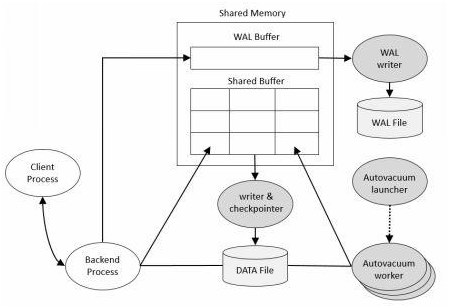
\includegraphics[width=0.8\textwidth]{image/theory/postgres_architecture.jpg}
    \caption{\textit{Kiến trúc tổng quan của PostgreSQL}}
    \label{fig:postgres-arch}
\end{figure}

Kiến trúc cốt lõi của PostgreSQL bao gồm các thành phần:
\begin{itemize}
    \item \textbf{Các tiến trình (Processes):} Điều phối toàn bộ hoạt động của cơ sở dữ liệu. Nó tiếp nhận kết nối, cấp phát tiến trình xử lý truy vấn cho từng client và duy trì các tác vụ chạy ngầm (ghi dữ liệu, dọn dẹp rác, sao lưu nhật ký).
    \item \textbf{Shared Memory:} Giúp tối ưu hóa hiệu suất truy xuất và tính toán. Thành phần này dùng vùng nhớ chung để đệm dữ liệu (giảm tải đọc/ghi ổ cứng) và cấp phát vùng nhớ riêng cho từng tiến trình để thực hiện các phép toán phức tạp như sắp xếp hay gộp bảng.
    \item \textbf{Storage Manager::} Lưu trữ vật lý và bảo vệ dữ liệu. Nó ghi lại dữ liệu thực tế của các bảng/chỉ mục vào ổ cứng và duy trì nhật ký giao dịch (Write-AHead Logs) để đảm bảo không mất mát dữ liệu và cho phép phục hồi khi hệ thống gặp sự cố.
\end{itemize}

PostgreSQL là lựa chọn tốt cho các ứng dụng cần độ tin cậy cao và tính năng
mạnh mẽ. Đối với các hệ thống đơn giản hơn hay có scale lớn hơn, chúng ta
nên cân nhắc sử dụng MySQL hoặc NoSQL thay cho Postgres.

\subsection{Redis}
Redis (Remote Dictionary Server) là một hệ quản trị cơ sở dữ liệu NoSQL mã nguồn mở, hoạt động theo cơ chế in-memory và lưu trữ dữ liệu dưới dạng cặp key–value. Các dặc điểm nổi bật có thể kể đến:
\begin{itemize}
    \item \textbf{In-memory}: Dữ liệu được lưu chủ yếu trên RAM nên thời gian phản hồi thường ở mức microsecond, phù hợp cho các hệ thống real-time.
    \item \textbf{Key-Value}: Mỗi khóa trỏ tới một giá trị. Các giá trị không chỉ là chuỗi đơn thuần mà có thể là nhiều cấu trúc dữ liệu phức tạp.
    \item \textbf{Tính bền vững dữ liệu}: Dù là in-memory, Redis vẫn có cơ chế ghi xuống đĩa (RDB snapshot, AOF log) để phục hồi dữ liệu khi khởi động lại hoặc gặp sự cố.
    \item \textbf{Mở rộng \& tích hợp}: Có thể chạy đơn node hoặc cụm (Redis Cluster), hỗ trợ nhiều ngôn ngữ lập trình qua client đa dạng.
\end{itemize}
Redis thường được sử dụng trong các vai trò:
\begin{itemize}
    \item \textbf{Cache}: Giảm tải cho database truyền thống bằng cách lưu kết quả truy vấn, session, hoặc dữ liệu đọc nhiều.
    \item \textbf{Cơ sở dữ liệu chính}: Cho các trường hợp cần tốc độ cao, dữ liệu có tính biến đổi lớn (leaderboard, realtime analytics, state của game).
    \item \textbf{Message broker / pub-sub}: Truyền dữ liệu thời gian thực giữa các service.
    \item \textbf{Hàng đợi}: Xử lý bất đồng bộ, job queue, delayed job.
\end{itemize}

\section{Các dịch vụ tích hợp}
\subsection{Dịch vụ thông báo và truyền thông thời gian thực}
\label{subsec:backend_notification_realtime}

Firebase Cloud Messaging (FCM) là nền tảng điện toán đám mây do Google cung cấp~\cite{fcm_doc}, hỗ trợ gửi thông báo đẩy và thông điệp dữ liệu đến ứng dụng trên thiết bị người dùng một cách tin cậy và tối ưu năng lượng pin. Bên cạnh đó, Socket.IO là thư viện hỗ trợ giao tiếp hai chiều thời gian thực dựa trên giao thức WebSocket~\cite{socketio_doc}, bảo đảm độ trễ truyền thông thấp.

Trong MyHCMUT Mobile, nhu cầu nhận biết các sự kiện phê duyệt đơn từ, văn bản mới và lịch họp đóng vai trò then chốt đối với trải nghiệm người dùng. Nhóm sử dụng FCM để tiếp nhận thông báo đẩy từ các dịch vụ backend và trích xuất siêu dữ liệu (metadata) đi kèm nhằm kích hoạt tính năng điều hướng sâu đến đúng màn hình nghiệp vụ liên quan. Đối với tính năng điểm danh cuộc họp trong phân hệ Lịch làm việc, nhóm khai thác Socket.IO để nhận các cập nhật trạng thái tức thời giữa thiết bị di động và phòng họp máy chủ.